\documentclass[a4paper]{article}

\usepackage[portuguese]{babel}
\usepackage{comment}
\usepackage[T1]{fontenc}
\usepackage[utf8]{inputenc}
\usepackage{hyperref}
\usepackage{graphicx}
\usepackage{float}
\usepackage{multirow}
\usepackage[hypcap]{caption} % makes \ref point to top of figures and tables
\usepackage{amsmath}
\usepackage{multicol} %for page layout on section Maximização do Throughput
%\usepackage[usenames,dvipsnames,svgnames,table]{xcolor}
\usepackage{pdflscape}	% landscape pages
\usepackage{subcaption}

\begin{document}

\begin{titlepage}

\begin{center}


\includegraphics[width=6cm]{./title}\\[3cm]

\textsc{\LARGE Projecto de Sistemas Digitais}\\[1.5cm]

\textsc{\Large Laboratório 2}\\[1.5cm]


{ \huge \bfseries Escalonamento e Partilha de Recursos \\[3cm] }


\noindent
\begin{minipage}{0.4\textwidth}
\begin{flushleft} \large
Rafael Gonçalves, 73786
\end{flushleft}
\end{minipage}
\begin{minipage}{0.4\textwidth}
\begin{flushright} \large
Gonçalo Ribeiro, 73294
\end{flushright}
\end{minipage}

\vfill

{\large \today}


\end{center}

\end{titlepage}

\tableofcontents
\pagebreak

\section{Introdução}
O presente trabalho tem por objectivo o desenho e implementação de um processador dedicado para processamento morfológico de imagens binárias i.e.\ imagens cujos pixeis podem ter apenas dois valores distintos.

As operações a realizar sobre as imagens são cinco: erosão, dilatação, fecho (dilatação seguida de erosão), abertura (erosão seguida de dilatação) e extração de contornos (diferença entre a imagem original e a sua erosão).

O elemento estruturante considerado é um quadrado de $3\times3$ pixeis---por exemplo na operação de erosão analisa-se uma área $3\times3$ px centrada nesse pixel para decidir se o mesmo deve ser erodido.

As imagens consideradas têm no máximo $128\times128$ px. Uma imagem é transferida de um computador para a uma BRAM da FPGA via USB e o processador dedicado deve ler dessa BRAM de entrada e escrever a imagem transformada numa BRAM de saída. A imagem transformada é depois transferida de volta para o PC, onde pode ser visualizada.

O desempenho do circuito é avaliado pelo tempo de processamento dos dados entre as duas memórias.

\section{Formato das Imagens}
\label{sec:formato_imagens}
O formato das imagens não é definido no enunciado do projecto. É esperado que os alunos desenvolvam um formato de imagem que julguem mais adequado.

As imagens têm no máximo $128\times128\times1$ bits (2 kB), que é precisamente a dimensão de cada uma das 4 BRAMs existentes na FPGA XC3S-100E-4CP132. Como tal, no caso das imagens maiores, a BRAM de entrada é completamente preenchida, o que significa que não sobram bits para representar por exemplo as dimensões da imagem. Assim, essa informação não pode fazer parte do formato da imagem.

Decidiu-se então que as dimensões da imagem (largura e altura) são passadas ao processador dedicado fazendo uso dos 8 interruptores existentes na placa de desenvolvimento. Introduz-se primeiro a largura e pressiona-se um botão de pressão para armazenar essa dimensão. De seguida faz-se o mesmo para a altura.

A imagem é representada em memória sempre como 4 palavras de 32 bits por cada linha da imagem. Se a imagem tiver menos que 128 bits de largura é introduzido \textit{padding} que perfaça 128 bits. O \textit{padding} utilizado consiste na extensão do último bit válido de cada linha da imagem. Estas características foram escolhidas de forma a facilitar o processamento da imagem.

\section{Arquitectura}
% intro à arquitectura
As operações elementares (dilatação e erosão) podem ser realizadas em dois passos distintos: primeiro executa-se a operação apenas na horizontal, i.e. usando um elemento estruturante de dimensão $3\times1$; de seguida expande-se o resultado para a linha acima e abaixo.

A arquitectura projectada faz uso desta propriedade e como tal tem duas FSMDs principais. A primeira, que realiza alterações apenas na horizontal, é designada por \textit{Horizontal Alteration after Line Fetch} (HALF). A segunda faz a expansão vertical e chama-se \textit{Storing Alterations after Vertical Exchange} (SAVE). A \autoref{fig:poc} ilustra as duas fases de processamento.

\begin{figure}[h]
	\centering
	\begin{subfigure}[b]{0.32\textwidth}
		\centering
		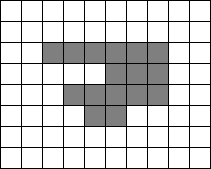
\includegraphics[width=\linewidth]{poc_orig}
		\caption{}
		\label{fig:por_orig}
	\end{subfigure}
	\begin{subfigure}[b]{0.32\textwidth}
		\centering
		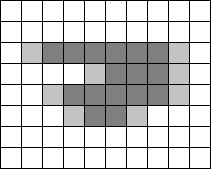
\includegraphics[width=\linewidth]{poc_HALF}
		\caption{}
		\label{fig:poc_HALF}
	\end{subfigure}
	\begin{subfigure}[b]{0.32\textwidth}
		\centering
		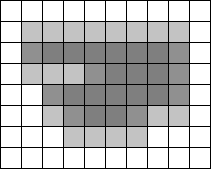
\includegraphics[width=\linewidth]{poc_SAVE}
		\caption{}
		\label{fig:poc_SAVE}
	\end{subfigure}
	\caption{Imagem (a) original (b) após HALF (c) após HALF e SAVE}
	\label{fig:poc}
\end{figure}

Para além dessas duas componentes principais do circuito existe ainda outra que é responsável por fazer o \textit{padding} de cada linha antes do armazenamento na BRAM de saída.

\subsection{HALF}
% intro ao HALF
HALF é responsável por fazer as transformações horizontais de cada linha da imagem, como exemplificado na \autoref{fig:poc_HALF}.

\subsubsection{Datapath}
A datapath da HALF tem por base dois módulos: um bloco de dilatação (D) e outro de erosão (E). Uma dilatação horizontal corresponde basicamente a fazer um \texttt{OR} de cada bit com o bit à sua esquerda e à sua direita; da mesma forma, uma erosão corresponde a um \texttt{AND}. Assim, os blocos D e E são \textit{arrays} dessas portas de forma a processar palavras 32 bits de cada vez. Existe, naturalmente, alguma lógica extra que é responsável por expansões de uma palavra para outra---por exemplo se uma imagem tiver como largura duas palavras de 32 bits a dilatação horizontal da primeira pode afectar o primeiro bit da segunda; e o primeiro bit da segunda pode afectar o último bit da primeira. O circuito dos blocos D e E pode ver-se na \autoref{fig:HALF_E_D_blocks}.

\begin{figure}[h]
	\centering
	\begin{subfigure}[b]{0.45\textwidth}
		\centering
		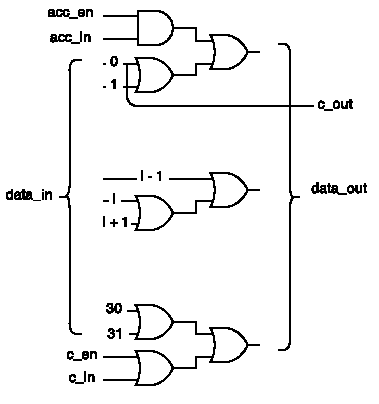
\includegraphics[width=\linewidth]{HALF_D_block}
		\caption{}
		\label{fig:HALF_D_block}
	\end{subfigure}
	\begin{subfigure}[b]{0.45\textwidth}
		\centering
		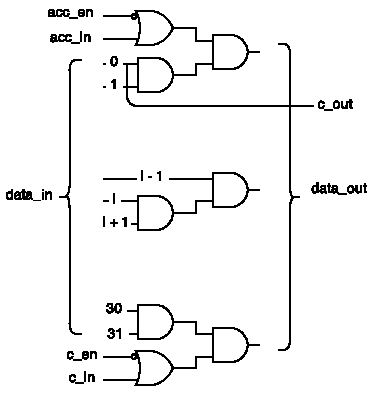
\includegraphics[width=\linewidth]{HALF_E_block}
		\caption{}
		\label{fig:HALF_E_block}
	\end{subfigure}
	\caption{(a) bloco de dilatação (b) bloco de erosão}
	\label{fig:HALF_E_D_blocks}
\end{figure}

%explicar carry e accum
A entrada \texttt{c\_in} permite que o MSB (\textit{most significant bit}) de uma palavra seja alterado tendo em conta o LSB (\textit{least significant bit}) da palavra anterior. Por outro lado, a entrada \texttt{acc\_in} permite que o LSB de uma palavra seja alterado tomando em consideração o MSB da palavra seguinte. As entradas \texttt{c\_en} e \texttt{acc\_en} permitem indicar se tanto \texttt{c\_in} como \texttt{acc\_in} têm valores válidos. Na primeira palavra de cada imagem \texttt{c\_en} deve estar a \texttt{0} e na última palavra \texttt{acc\_en} deve estar a \texttt{0}. Nos restantes casos esses sinais devem estar a \texttt{1}.

Poder usar o sinal \texttt{acc\_in} significa necessariamente que quando uma palavra é processada por um dos blocos da \autoref{fig:HALF_E_D_blocks} a palavra seguinte já tem que ter ser sido lida da memória. Para isso existe na arquitectura um registo \texttt{\_accum} para cada bloco. Este registo permite pôr a palavra $n$ em espera até que a palavra $n+1$ seja lida. Quando a palavra $n+1$ é lida tem-se toda a informação necessária ao processamento da palavra $n$. O mesmo registo põe em espera o \textit{c\_out} da palavra $n-1$ para que possa ser usado no processamento da $n$. Estes registos podem ser vistos na \autoref{fig:HALF_datapath}.

Outra particularidade da datapath da HALF é que para realizar as operações compostas o output das operações elementares pode ser redireccionado para a entrada do bloco complementar. Assim um fecho horizontal pode ser calculado passando \texttt{data\_in} pelo bloco D e redireccionando o output para a entrada do bloco E. À saída teremos o fecho horizontal da palavra em \texttt{data\_in}.

Para que o redireccionamento de uma palavra de um bloco para outro não criasse um caminho crítico dentro do bloco introduziu-se um registo \texttt{\_delay\_reg} à saída dos blocos D e E. Estes registos permitem que nas operações de abertura e fecho se faça armazenamento do resultado intermédio para que o caminho crítico não deva ser o percurso desde \texttt{data\_in} até ao \texttt{data\_out} passando pelo segundo bloco.

Devido aos atrasos causados pelos registos \texttt{\_accum} e \texttt{\_delay\_reg} é necessário fazer uma compensação---i.e.\ um atraso---dos sinais de controlo da datapath. Para isso os sinais de controlo \texttt{\_carry\_en} e \texttt{\_accum\_en} são passados por um ou dois registos conforme se trate, respectivamente, de uma operação elementar ou de uma composta. Esse atraso variável é controlado pelos sinais \texttt{\_delay}.

Paralelamente à saída \texttt{output\_func} existe também a \textit{bus} \texttt{output\_orig} que é a palavra original correspondente à palavra transformada durante a HALF. A palavra original é usada apenas durante a SAVE e somente na operação de extracção de contornos. A palavra original é atrasada fazendo uso do registo \texttt{d\_accum\_en}, que não é usado para outro fim durante extracções de contornos. Assim, a palavra original e transformada saem da datapath sincronizadas.

O diagrama da datapath da HALF está patente na \autoref{fig:HALF_datapath}. Não são representados sinais de relógio.

\begin{figure}[H]
	\centerline{
		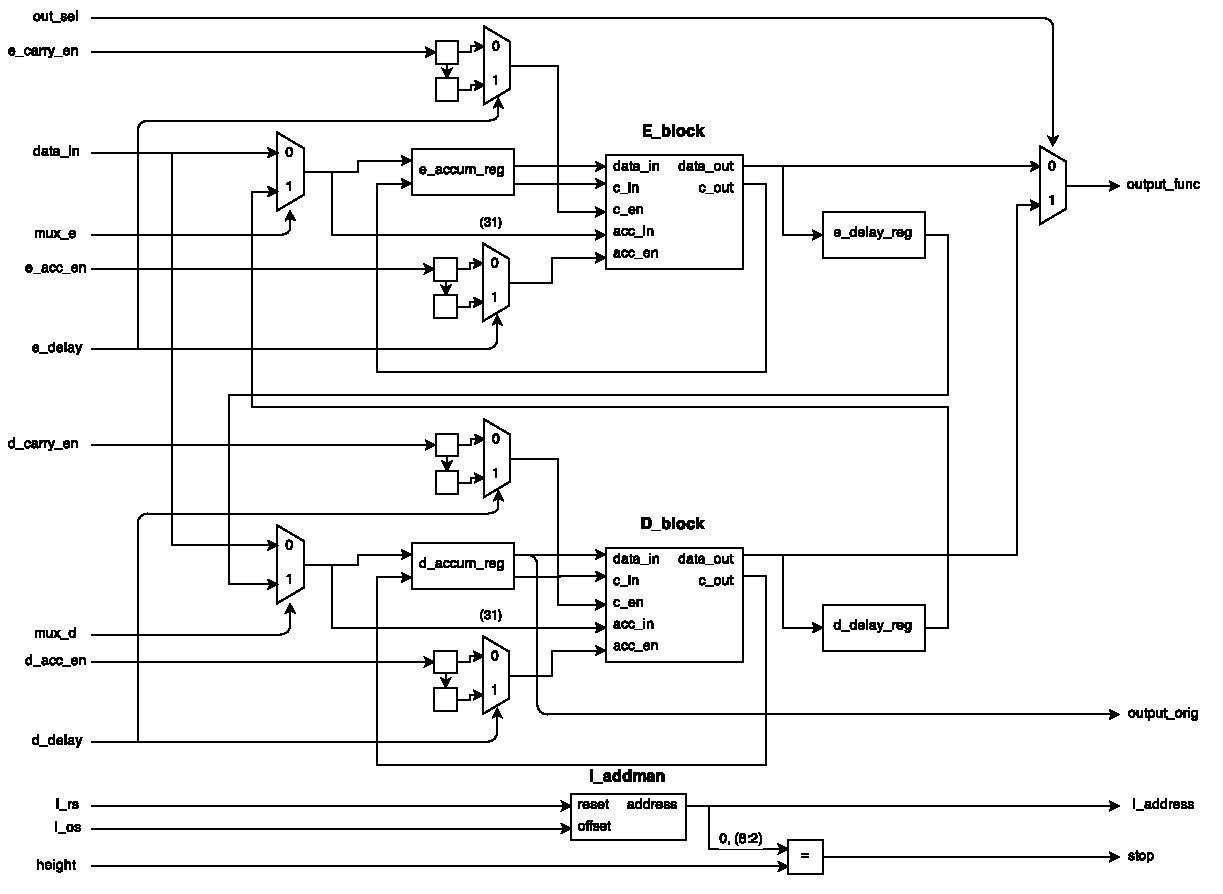
\includegraphics[width=.95\paperwidth]{HALF_datapath}
	}
	\caption{Datapath da HALF}
	\label{fig:HALF_datapath}
\end{figure}

O bloco \texttt{i\_addman} é o \textit{address manager} da BRAM de entrada. Este bloco é um contador que regista qual o endereço a ser lido da BRAM de entrada. Com base no endereço actual e na altura da imagem é possível calcular o sinal \texttt{stop}, que indica à FSM se o trabalho da HALF terminou.

\subsubsection{FSM}
A máquina de estados da HALF pode ser vista na \autoref{fig:HALF_FSM}.

\begin{figure}
	\centering
	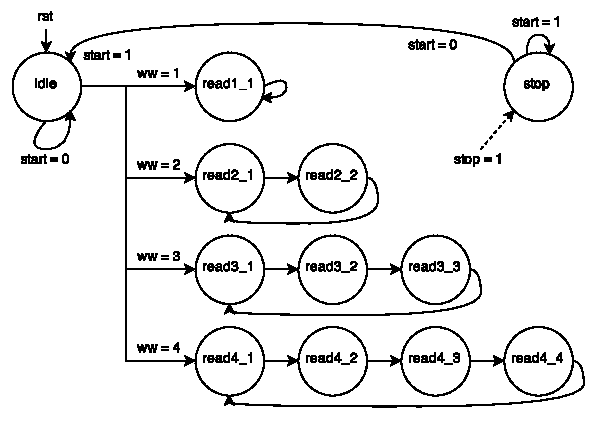
\includegraphics[width=0.8\linewidth]{HALF_FSM}
	\caption{Máquina de estados da HALF}
	\label{fig:HALF_FSM}
\end{figure}

Existem duas classes de outputs nesta máquina de estados: uns dependem apenas do estado actual, sendo independentes do tipo de operação; os outros dependem apenas do tipo de operação. Da primeira classe fazem parte os \textit{enables} dos blocos D e E, reset do \texttt{addman}, offset da BRAM de entrada e o offset da unidade de armazenamento do SAVE. Da outra classe fazem parte os sinais de controlo de multiplexers e os sinais de \textit{delay}.

Para a primeira palavra de cada linha o \textit{carry enable} é desactivado, visto que o \textit{carry} nesse caso se refere a uma palavra da linha anterior. O \textit{accumulator enable} é desactivado para a última palavra de cada linha visto que nesse caso \texttt{acc\_in} se refere à primeira palavra da linha seguinte.

Os sinais de controlo dos multiplexers à entrada dos blocos D e E e o do mux de saída são alterados de acordo com a operação a executar. Nas operações compostas há que redireccionar a saída de um dos blocos para a entrada do outro. Para além disso numa opção composta há que activar o sinal de \textit{delay} de forma a atrasar o \textit{carry enable} e \textit{accumulator enable} do segundo bloco a actuar.

O sinal de \textit{reset} do \texttt{addman} é activado apenas no estado \texttt{idle}. O sinal de \textit{offset} é gerado de forma a saltar palavras da memória que contenham apenas \textit{padding}.

%\begin{table}
%\small
%\centerline{
%\begin{tabular}{|c||c|c|c|c|c|c|c|c|c|c|c|c|}
%\hline 
%& idle & read1\_1 & read2\_1 & read2\_2 & read3\_1 & read3\_2 & read3\_3 & read4\_1 & read4\_2 & read4\_3 & read4\_4 & stop\\ 
%\hline 
%\hline
%mux\_e & • & • & • & • & • & • & • & • & • & • & • & • \\ 
%\hline 
%mux\_d & • & • & • & • & • & • & • & • & • & • & • & • \\ 
%\hline 
%e\_carry\_en & • & • & • & • & • & • & • & • & • & • & • & • \\ 
%\hline 
%d\_carry\_en & • & • & • & • & • & • & • & • & • & • & • & • \\ 
%\hline 
%e\_acc\_en & • & • & • & • & • & • & • & • & • & • & • & • \\ 
%\hline 
%d\_acc\_en & • & • & • & • & • & • & • & • & • & • & • & • \\ 
%\hline 
%e\_delay & • & • & • & • & • & • & • & • & • & • & • & • \\ 
%\hline 
%d\_delay & • & • & • & • & • & • & • & • & • & • & • & • \\ 
%\hline 
%i\_rs & • & • & • & • & • & • & • & • & • & • & • & • \\ 
%\hline
%i\_en & • & • & • & • & • & • & • & • & • & • & • & • \\ 
%\hline 
%i\_os & • & • & • & • & • & • & • & • & • & • & • & • \\ 
%\hline 
%f\_os & • & • & • & • & • & • & • & • & • & • & • & • \\ 
%\hline 
%\end{tabular}
%}
%\caption{sinais de saída da FSM para cada estado}
%\label{tab:HALF_FSM_outputs}
%\end{table}

\subsection{SAVE}
% intro ao SAVE

O módulo SAVE recebe a imagem já processada horizontalmente, e procede à sua ``expansão'' na vertical. Para isto precisa de três palavras (correspondentes às linhas actual, anterior e seguinte).

\subsubsection{Datapath}
\label{sssec:SAVE_Datapath}
Para ter disponíveis as ditas três palavras, que estão separadas entre si por 3 outras palavras, é necessário uma unidade de armazenamento algo particular. O conceito para esta unidade está representado na \autoref{fig:SAVE_storageunit_1}.

\begin{figure}[h]
	\centering
	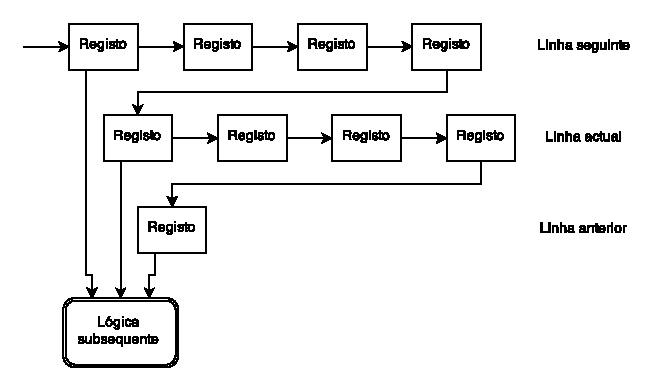
\includegraphics[width=0.8\linewidth]{SAVE_storageunit_1}
	\caption{Unidade de Armazenamento do módulo SAVE}
	\label{fig:SAVE_storageunit_1}
\end{figure}

No entanto, uma vez que o módulo HALF salta os blocos de padding, o conceito foi expandido de maneira a permitir ``saltos''. Assim, o que foi implementado está representado na \autoref{fig:SAVE_storage_unit_wmux}.

\begin{figure}[h]
	\centering
	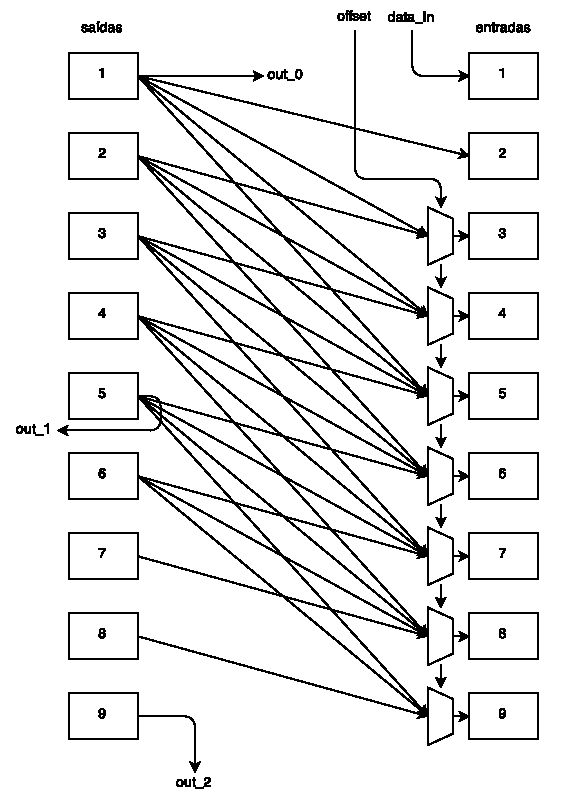
\includegraphics[width=0.8\linewidth]{SAVE_storage_unit_wmux}
	\caption{Unidade de Armazenamento do módulo SAVE revista}
	\label{fig:SAVE_storage_unit_wmux}
\end{figure}

Uma vez disponíveis as três palavras relevantes (ou duas, no caso da primeira e última palavra, que não têm antecessor nem sucessor, respectivamente), são sobre si efectuadas as operações lógicas correspondentes à operação morfológica a realizar sobre a imagem (ver \autoref{fig:SAVE_datapath_E_D}).

\begin{figure}[h]
	\centering
	\begin{subfigure}[b]{0.45\textwidth}
		\centering
		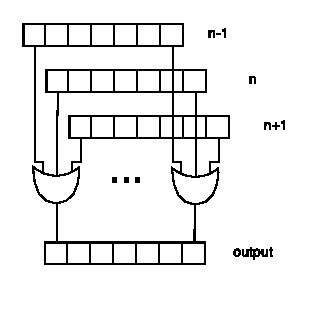
\includegraphics[width=\linewidth]{SAVE_datapath_D}
		\caption{Dilatação}
		\label{fig:SAVE_datapath_D}
	\end{subfigure}
	\begin{subfigure}[b]{0.45\textwidth}
		\centering
		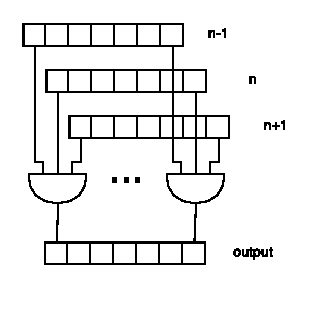
\includegraphics[width=\linewidth]{SAVE_datapath_E}
		\caption{Erosão}
		\label{fig:SAVE_datapath_E}
	\end{subfigure}
	\caption{Unidades funcionais da Datapath do SAVE}
	\label{fig:SAVE_datapath_E_D}
\end{figure}

Estes blocos são dispostos na arquitectura especificada na \autoref{fig:SAVE_Datapath}, de maneira a realizar as várias operações.

Caso a operação seja simples, o resultado do módulo HALF é direccionado para a unidade de armazenamento principal, e a sua saída para os blocos lógicos, cujo resultado vai para a saída.

No caso de ser uma operação composta (abertura ou fecho), a saída da primeira operação é redireccionada para uma segunda unidade de armazenamento, a partir da qual é realizada a última operação antes do armazenamento na memória.

Finalmente, caso a operação seja detecção de limites, a imagem erodida horizontalmente é direccionada para a unidade de armazenamento principal, e posteriormente erodida verticalmente. Simultaneamente, a imagem original, inalterada, é direccionada para a segunda unidade de armazenamento, cuja saída é direccionada para o bloco de Subtracção, cuja única operação é uma \texttt{XOR} bit-a-bit entre os dois operandos.

\begin{figure}[h]
	\centering
	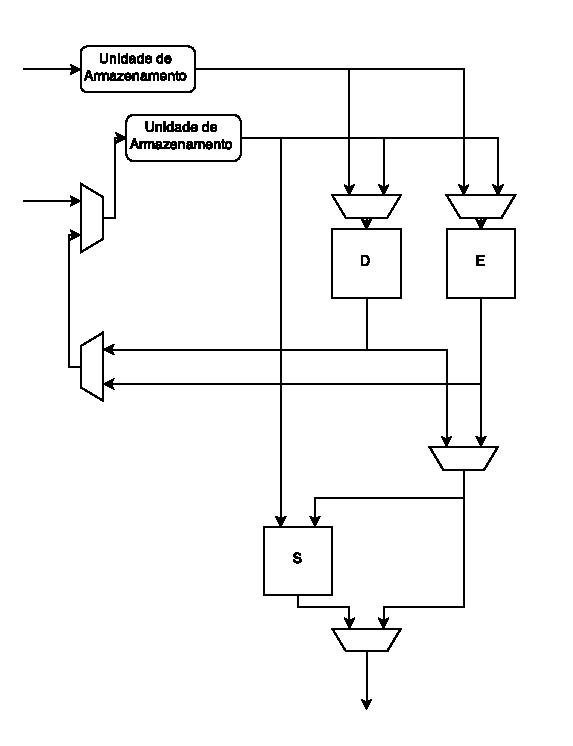
\includegraphics[width=0.6\linewidth]{SAVE_Datapath}
	\caption{Datapath do módulo SAVE}
	\label{fig:SAVE_Datapath}
\end{figure}

\subsubsection{FSM}

A máquina de estados que controla o módulo SAVE pode ser observada na \autoref{fig:SAVE_fsm}. A máquina de estados apenas distingue o primeiro ciclo dos restantes, uma vez que no primeiro ciclo é necessário forçar o barramento correspondente à palavra anterior à actualmente processada de maneira a não ``contaminar'' as informações relativas à palavra actual e à seguinte com os dados de um registo não inicializado.

\begin{figure}[h]
	\centering
	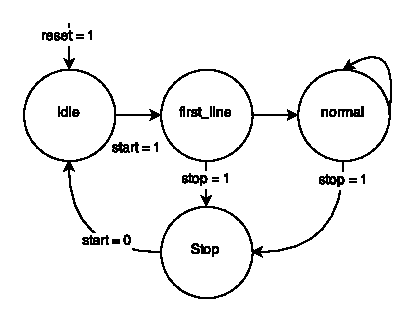
\includegraphics[width=0.6\linewidth]{SAVE_fsm}
	\caption{Máquina de estados do módulo SAVE}
	\label{fig:SAVE_fsm}
\end{figure}

Quanto à distinção de operações, esta é feita via os três bits de controlo que especificam a operação, que determinam qual o percurso dos dados no interior do módulo.

Se se tratar de uma erosão ou de uma dilatação, o multiplexer à entrada do bloco correspondente selecciona a Unidade de Armazenamento principal, o multiplexer de função selecciona a saída desse mesmo bloco, e o multiplexer de saída selecciona o \textit{output} do multiplexer de função.

No caso de uma abertura ou fecho, um multiplexer de entrada dos blocos é configurado para a unidade de armazenamento principal, o outro para a secundária, e as saídas desses blocos são configuradas para a unidade secundária e para o \textit{output}, respectivamente.

Finalmente, no caso de uma Extracção de Contornos, a configuração é idêntica à de uma erosão, excepto pelo facto de que a imagem original é direccionada para a Unidade de Armazenamento secundária, e o \textit{output} provém do bloco de subtracção (isto é, à operação \texttt{XOR} -- os bits iguais entre as imagens são apagados, e os diferentes marcados).

\subsection{\textit{Padder}}
% intro ao padder
Visto que o formato de imagem desenvolvido usa como \textit{padding} a extensão do último bit válido há que gerar esse \textit{padding} antes de fazer o armazenamento na BRAM de saída. Para além disso há que acrescentar palavras que tenham sido suprimidas durante o processamento (i.e.\ palavras constituídas somente por \textit{padding}). São estas as funções do \textit{padder} descrito nesta secção.

\subsubsection{Datapath}
O \textit{padder} recebe palavras de 32 bits. Para fazer o \textit{padding} é necessário aceder ao último bit válido de uma linha. Esse bit pode estar em qualquer uma de 4 palavras de 32 bits que constituem a linha. Para obter o bit de interesse usa-se um mux de 32 entradas.

O número de bits da palavra de entrada que passam para a palavra de saída depende da largura da imagem. Como tal, existe uma espécie de descodificador que selecciona que bits da palavra de entrada devem passar intocados. Os bits da palavra que não passarem são substituídos pelo bit de \textit{padding}.

Há palavras de saída que serão compostas apenas pelo bit de \textit{padding}. Para que isso seja possível o bit de \textit{padding} é guardado num registo para que possa ser usado nas palavras subsequentes da mesma linha.

O esquema da datapath do \textit{padder} descrito está patente na \autoref{fig:padder_datapath}.

\begin{figure}[h]
	\centering
	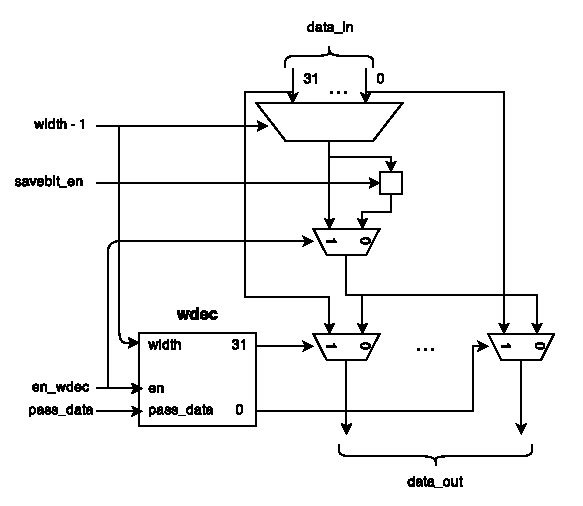
\includegraphics[width=.8\linewidth]{padder_datapath}
	\caption{Datapath do \textit{padder}}
	\label{fig:padder_datapath}
\end{figure}

\subsubsection{FSM}
A máquina de estados do \textit{padder} é uma máquina de Moore e consta na \autoref{fig:padder_FSM}.

Nos estados representados a amarelo toda a informação da palavra é informação válida e portanto a palavra passa intocada. Nos estados a verde o último bit válido encontra-se algures nessa palavra e portanto é feita extensão desse bit e o mesmo é guardado no registo da datapath. Nos estados a azul todos os bits à saída são \textit{padding}, com o mesmo valor do bit guardado no estado a verde anterior. O processo de \textit{padding} repete-se para todas as linhas, até que o sinal \texttt{stop} seja activado.

\begin{figure}[h]
	\centering
	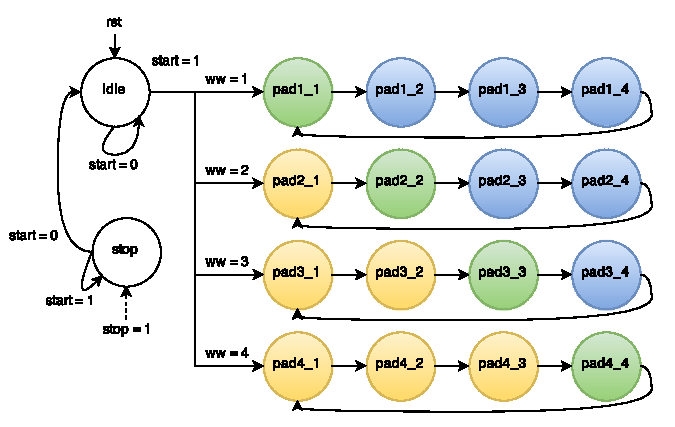
\includegraphics[width=.9\linewidth]{padder_FSM}
	\caption{Máquina de estados do \textit{padder}}
	\label{fig:padder_FSM}
\end{figure}

\subsection{União dos módulos}

Uma vez desenhados os três módulos componentes da arquitectura, é necessário ligá-los entre si.

O módulo SAVE recebe como entradas alguns sinais de controlo, provenientes da interface com o utilizador (interruptores e botões da placa \textit{Basys2}), e os \textit{outputs} do módulo HALF.

Por sua vez, os resultados do SAVE deveriam ser utilizados pelo módulo de \textit{padding} para completar as lacunas com a extensão do bit relevante. No entanto, devido às limitações de tempo, esta ligação não foi implementada em VHDL.

Alguns dos sinais de controlo ou endereços correspondem apenas ao atraso de outros sinais, pelo que o circuito que instancia os vários módulos tem também uma série de registos, de maneira a fazer este atraso.

\section{\textit{Performance}}	% titulo melhor ?
%A aquitectura desenhada processa as imagens com complexidade $O(m)$, sendo $m$ o número de linhas da imagem.

A HALF tem tempo de processamento proporcional ao número de palavras da imagem que não sejam constituídas exclusivamente por \textit{padding}, ou seja tem complexidade $O(w m)$, em que $w$ é o número de palavras que não são \textit{padding} e $m$ é o número de linhas da imagem. Cada ciclo de execução processa uma palavra, sendo que as operações compostas custam apenas mais um ciclo que as elementares.

A SAVE processa com complexidade $O(w m)$. Mais uma vez esta unidade processa apenas palavras que não sejam exclusivamente \textit{padding}. O \textit{throughput} desta unidade é inferior a 1 palavra por ciclo visto que em imagens com largura superior a uma palavra de 32 bits há que esperar que a unidade de armazenamento da SAVE seja preenchida até que existam palavras correspondentes de linhas seguidas. As operações compostas podem demorar até mais 4 ciclos do que as operações elementares.

Do \textit{padder} saem $4\times m$ resultados independentemente do valor de $w$, devido à expansão das linhas para 4 palavras de forma a que seja respeitado o formato definido para a imagem na \autoref{sec:formato_imagens}. No entanto é possível acelerar a escrita na BRAM de saída de forma a que as palavras de \textit{padding} sejam escritas mais rapidamente que as restantes, fazendo com que o \textit{padder} não seja um ponto de ``engarrafamentos''.

Tendo em conta que as imagens a serem processadas têm no máximo 128 bits de largura, ou seja $w=4$, a complexidade da arquitectura desenhada é na sua totalidade $O(m)$, em que $m$ é o número de linhas da imagem.

Cada um dos 3 blocos principais da arquitectura foi sintetizado e a frequência máxima de cada bloco é mostrada na \autoref{tab:freqs_operacao}. O módulo mais lento é o SAVE.

\begin{table}
\centering
\begin{tabular}{|c|c|}
\cline{2-2}
\multicolumn{1}{c|}{} & Frequência Máxima \\ 
\cline{2-2}
\hline
HALF & 167 MHz \\ 
\hline 
SAVE & 115 MHz \\ 
\hline 
padder & 217 MHz \\ 
\hline 
HALF + SAVE & 109 MHz \\ 
\hline 
\end{tabular} 
\caption{Frequência máxima de operação dos módulos da arquitectura}
\label{tab:freqs_operacao}
\end{table}

% HALF
%   Minimum period: 5.968ns (Maximum Frequency: 167.560MHz)
%   Minimum input arrival time before clock: 4.963ns
%   Maximum output required time after clock: 6.890ns
%   Maximum combinational path delay: 5.885ns

% SAVE
%   Minimum period: 8.686ns (Maximum Frequency: 115.133MHz)
%   Minimum input arrival time before clock: 7.343ns
%   Maximum output required time after clock: 6.977ns
%   Maximum combinational path delay: 5.634ns

% padder 
%	Minimum period: 4.596ns (Maximum Frequency: 217.580MHz)
%	Minimum input arrival time before clock: 4.309ns
%	Maximum output required time after clock: 7.953ns
%	Maximum combinational path delay: 8.057ns

% HALF + SAVE
%   Minimum period: 9.159ns (Maximum Frequency: 109.182MHz)
%   Minimum input arrival time before clock: 9.426ns
%   Maximum output required time after clock: 6.822ns
%   Maximum combinational path delay: 7.058ns


\section{Visualizador}

De maneira a produzir ficheiros binários com imagens, foi programado em \texttt{C} um visualizador/editor de imagens binárias (recorrendo à biblioteca gráfica \emph{Allegro}).

O visualizador em questão foi produzido antes da introdução do \textit{padding} no formato, pelo que para ser utilizado na encarnação actual do projecto precisaria de alterações adicionais.

O visualizador recebe como parâmetros a largura e altura da imagem, e o nome do ficheiro. Caso exista, é mostrado e pode ser editado. Caso não exista, é criado um buffer inicializado a zeros, que pode posteriormente ser gravado.

\section{Conclusões e Comentários}

Infelizmente, não foi possível concluir o projecto devido a limitações temporais.

O processo foi desafiante e estimulante. A premissa do projecto motivou e levou à descoberta de alternativas de melhor performance.

Inicialmente, estava previsto fazer várias leituras e armazenar os seus resultados em registos sobre os quais seriam feitas as operações lógicas.

Eventualmente descobriu-se o facto de que as componentes horizontais e verticais podem ser executadas separadamente, e a arquitectura foi dividida em duas.

A utilização de \textit{padding} no formato de imagem foi motivado pelas complexidades implicadas pelas quebras de linha. No entanto, o formato de saída teria de ser o mesmo, pelo que a componente de \textit{padding} introduziu um novo elemento na arquitectura.

Os diversos módulos da arquitectura não foram unidos, nem foi feita a interface com a placa, muito menos o seu teste.

No caso de ser feita uma adenda ao projecto e à arquitectura, serão feitas as seguintes alterações:

\begin{itemize}
        \item A Unidade de Armazenamento descrita em \ref{sssec:SAVE_Datapath} e representada na \autoref{fig:SAVE_storage_unit_wmux} é desnecessariamente complexa, a sua única funcionalidade é prevenir um pequeno atraso \textit{overhead} (de entre 1 a 3 ciclos) nas situações em que há padding.

No entanto este ganho não é suficiente para justificar o elevado custo de hardware de todos os multiplexers extra. Esta Unidade de Armazenamento seria substituída pelo conceito simplificado da \autoref{fig:SAVE_storageunit_1}.

        \item Os atrasos necessários para os sinais entre os diversos módulos devem ser feitos de maneira consistente e coerente.

        \item Colocando um registo entre o bloco de erosão e o bloco de subtracção diminuiria o caminho crítico, pelo que aumentaria a frequência, e, consequentemente, a \textit{performance} do projecto.

\end{itemize}



\end{document}